\documentclass[]{article}
%\usepackage[latin1]{inputenc}
\usepackage[utf8]{inputenc}
\usepackage{float}
% Esto es para que el LaTeX sepa que el texto está en español:
%\usepackage[spanish]{babel}

% Paquetes de la AMS:
\usepackage{amsmath, amsthm, amsfonts}
\usepackage{graphicx}

%opening
\title{Trabajo Práctico 1}
\author{Jairo Jiménez \\
	Sergio De Raco}

\begin{document}

\maketitle


\section*{Objetivo}
El objetivo del presente trabajo es analizar las característcas en las cuáles el algoritmo J48 es robusto. El algoritmo será aplicado sobre la base de datos Latinobarómetro \cite{Latinobarometro2011}, la cual es una encuesta de percepción política, democrática y social de latinoamérica. Para poder observar las cualidades y deficiencias del algoritmo, este será sometido a diferentes tipos de pruebas para analizar su comportamiento.

\section*{Alcance}

Los datos utilizados provienen de la última encuesta disponible sin suscripción (año 2011) de [Latinobarómetro]<http://www.latinobarometro.org>, un estudio de opinión pública que realiza anualmente alrededor de 20.000 entrevistas en 18 países de América Latina. Los datos se encuentran disponibles online, junto con el cuestionario y la metodología correspondientes.
La encuesta se realiza en centros urbanos de los países de cobertura y contiene preguntas y datos acerca de la situación social, política y económica (actual, pasada y futura), distribución del ingreso, nivel educativo, percepciones acerca de la participación del Estado e información demográfica.

En este trabajo se seleccionaron variables (preguntas de la encuesta) que pudieran aportar a predecir la respuesta a la pregunta (P10ST):  ¿Cree usted que el país está o no progresando? Para ello se seleccionaron los siguientes atributos: 

% fijate si queres poner esta tabla
\begin{center}
	\begin{tabular}{|l|l|c|}\hline
		Descripción & Variable & \# Categ.\\ \hline
		Autopercepción de clase social & S14 & 6\\
		Estado civil & S15 & 4\\
		Sexo & S16 & 2\\
		Edad & S17 & N\\
		Propiedades y bienes & S28D & 3\\
		Satisfacción con la propia vida & P1ST & 5\\
		Situación económica actual & P3ST.A & 5\\
		Situación política actual & P3ST.B & 5\\
		Situación económica últimos 12 meses & P4ST & 5\\
		Percepción del nivel de (des)igualdad del ingreso & P12ST & 5\\
		Preferencia por la democracia & P13ST & 4\\
		Mejora en la democracia del país & P15N & 4\\
		Gobierno de pocos ó del pueblo & P19ST & 3\\
		Expectativa de mejora en el nivel educativo a futuro & P28NE & 4\\
		Nivel percibido de deomcracia en el país & P49ST.A & 4\\
		Orientación política declarada & P76ST & 4\\
		Fortaleza del Estado & P65ST & 3\\
		Situación económica personal y familiar & P6ST & 6\\
		Percepción de magnitud de futuras alzas de precios & S1NICC7 & 4\\ \hline
	\end{tabular}
\end{center}


La base completa contiene 20.204 registros y 414 columnas, que representan las preguntas y datos de la encuesta. Para el trabajo se seleccionaron respuestas por países sudamericanos (Argentina, Bolivia, Brasil, Chile, Colombia, Ecuador, Paraguay, Perú, Uruguay y Venezuela), así se redujo a 11.614 observaciones para las 20 variables. En primer lugar, se procedió a transformar la variable de clase (P10ST) en una variable binaria que en el dataset aparece relativamente balanceada, con participaciones de 43.5 y 56.5 en cada categoría. Luego, en los atributos seleccionadso se agregaron categorías para evitar introducir un sesgo en la poda sobre atributos con menor cantidad de categorías. 

\section*{Resultados esperados}
Los resultados esperados para cada uno de los temas a trabajar en este trabajo son:
\begin{itemize}
	\item Confianza: Sobreajuste a partir de algún valor de confianza, el performance en el grupo de training se aleja del performance en el grupo de test.
	\item Faltantes: Robustez cuando el árbol tiene pocos faltantes en todas las variables o faltantes sobre una sola variable. Sobreajuste cuando la imputación se hace teniendo en cuenta la clase y poco poder predictivo cuando la imputación se hace de manera global.
	\item Ruido: Poco poder predictivo del árbol en la medida que la cantidad de Ruido aumenta.
	\item Discretización: Robustez cuando la variable numérica no es buen discriminador. Sobre ajuste cuando la variablee numérica adquiere poder predictivo.
\end{itemize}

\section*{Metodología}
Para la realización del presente trabajo, se utiliza el sofware de minería de datos Weka \cite{Weka1} mediante el lenguaje estadístico R \cite{RCran} usando el paquete RWeka \cite{RWeka}. Para cada punto se programaron funciones que llaman a distintos comandos de Weka desde R con el vector de parámetros de control adecuado.



\section{Sobreajuste y poda}
Como primer paso se generó una familia de datasets variando el factor de confianza como función de poda en el rango $[0,0.5]$ a incrementos de 0.025. El mejor ajuste del árbol se observa cuando la confianza es de 0.1, luego comienza el sobreajuste del árbol, pues este deja baja la capacidad de pronosticar las nuevas instancias de manera correcta.\\
A medida que aumenta la confianza, aumentan el tamaño y el número de hojas Figura \ref{1.P1Conf}.


%\begin{figure}
%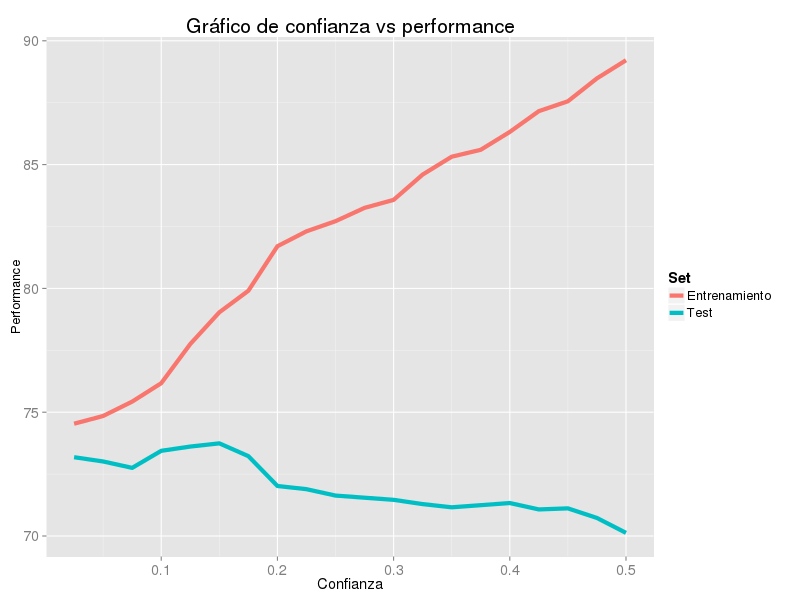
\includegraphics[width=0.8\linewidth,height=0.4\textheight]{Punto_1_Confianza_VS_ajuste}
%\caption[Confianza vs ajuste]{Confianza vs Ajuste}
%\label{P1ConfVSAjus}
%\end{figure}

\begin{figure}[H]
	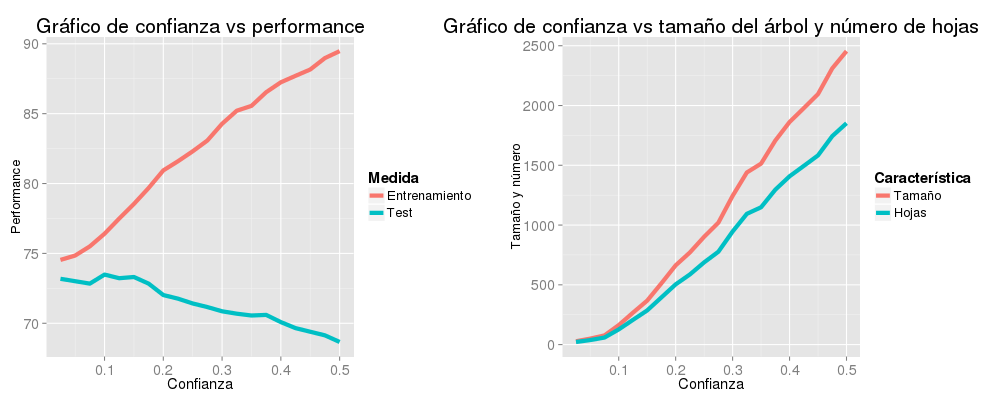
\includegraphics[scale = 0.4]{1_3_Conf_Perf_Num}
	\caption[Confianza vs ajuste]{Gráficos de confianza}
	\label{1.P1Conf}
\end{figure}
%
%
%\begin{figure}
%	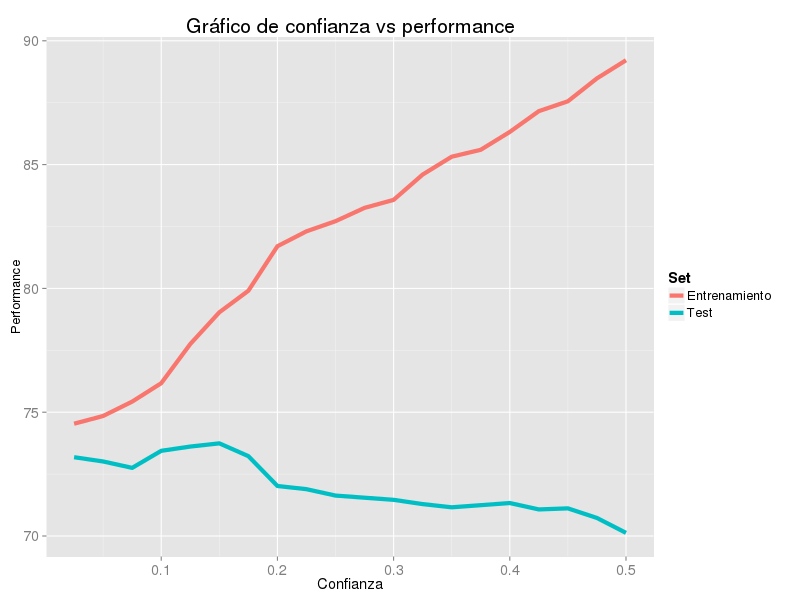
\includegraphics[scale = 0.4]{Punto_1_Confianza_VS_ajuste}
%	\caption[Confianza vs ajuste]{Confianza vs Ajuste}
%	\label{P1ConfVSAjus}
%\end{figure}

%\begin{figure}
%	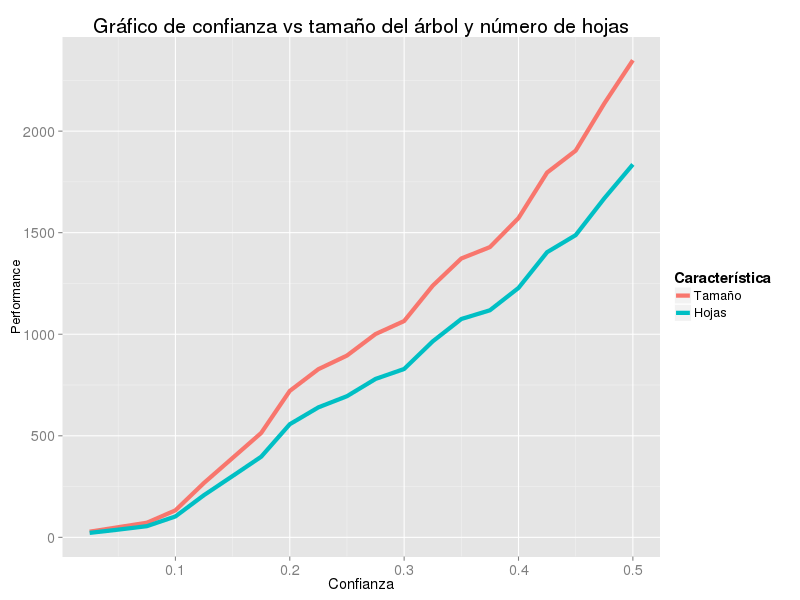
\includegraphics[scale = 0.4]{Punto_1_Confianza_VS_tamano}
%	\caption[Confianza vs ajuste]{Confianza vs Tamaño}
%	\label{P1ConfVSTamano}
%\end{figure}





\section{Tratamiento de datos faltantes}
Para el análisis de datos faltantes, el algoritmo se sometió a 3 diferentes tipos de faltantes sobre el conjunto de datos. Primero se analizó el efecto de los datos faltantes sobre una sola columna, luego sobre varias columnas pero solamente induciendo un faltante por fila y por último sobre varias columnas pero induciendo varios faltantes por fila. En los 3 casos, la cantidad de datos faltantes fue aumentando de 0 a 85\%.\\
Para lograr lo propuesto anteriormente, se programaron una serie de funciones que incrementan en 2.5\% el porcentaje de valores faltantes desde 0\% hasta 85\%, luego se imputaron los datos faltantes usando la moda (media) global o la moda (media) teniendo en cuenta la clase. Con cada set de datos, se calculó un nuevo árbol de clasificación y se tomaron los valores correspondientes para los análisis que se presentan a continuación.

\subsection{Sobre una sola variable}
En el caso de una variable, se seleccionó como candidata la variable que separa mejor el árbol (P15N).

\begin{figure}[H]
	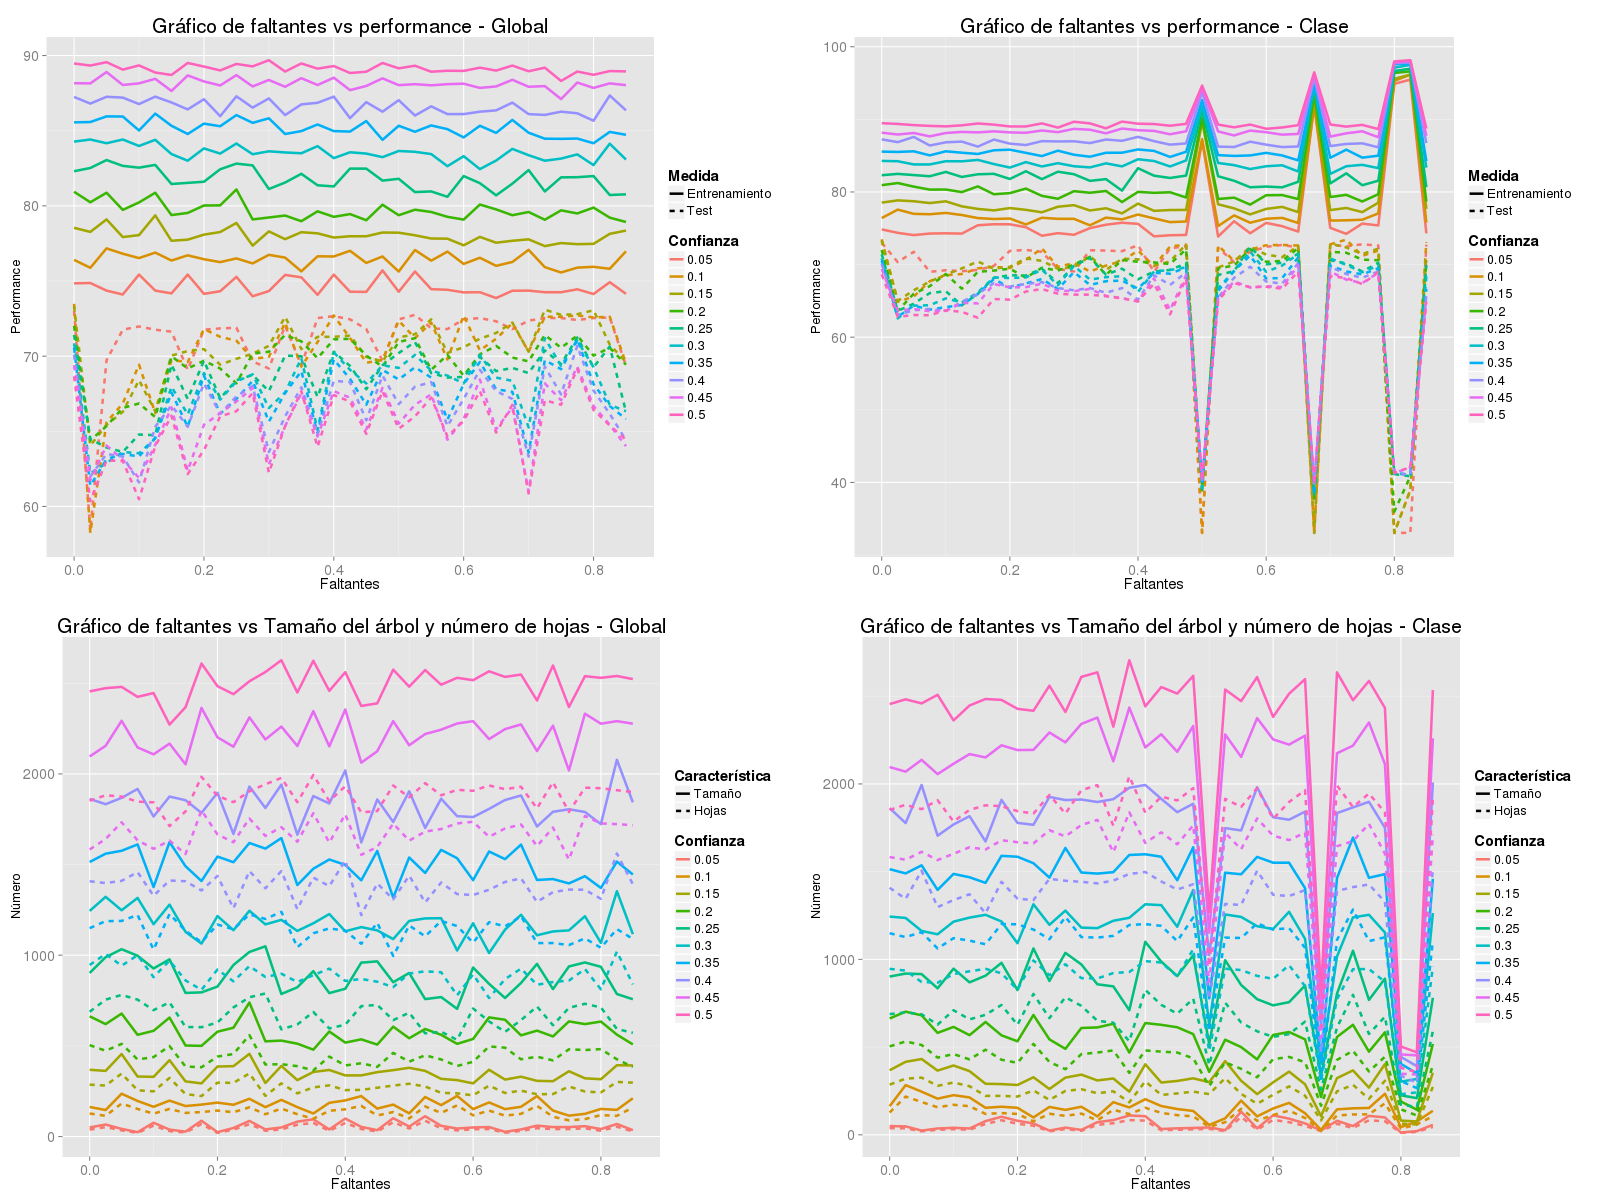
\includegraphics[scale = 0.27]{2_1_Unic_Col}
	\caption[Faltantes Unica variable]{Gráficos de Faltantes en una sola variable}
	\label{2.P2Unic_Var}
\end{figure}


\subsubsection{Imputación sin tener en cuenta la clase}
Cuando la imputación se hace sin tener en cuenta la clase, el árbol no se ve afectado por la variable imputada en el conjunto de entrenamiento. Ahora bien, en el conjunto de test, se nota que el performance cae, pero empieza a estabilizarse en la medida que la variable pierde poder discriminativo, hasta el punto en el que recupera el porcentaje de acierto.

\subsubsection{Imputación teniendo en cuenta la clase}

\subsection{Sobre varias variables con un único faltante por fila}
En este caso, se agregaron datos faltantes de manera aleatoria a las columnas, pero tengiendo en cuenta que solamente se admite un valor faltante por fila en el conjunto de datos. Figura \ref{2.P2MultVarUnicFil} 

\begin{figure}[H]
	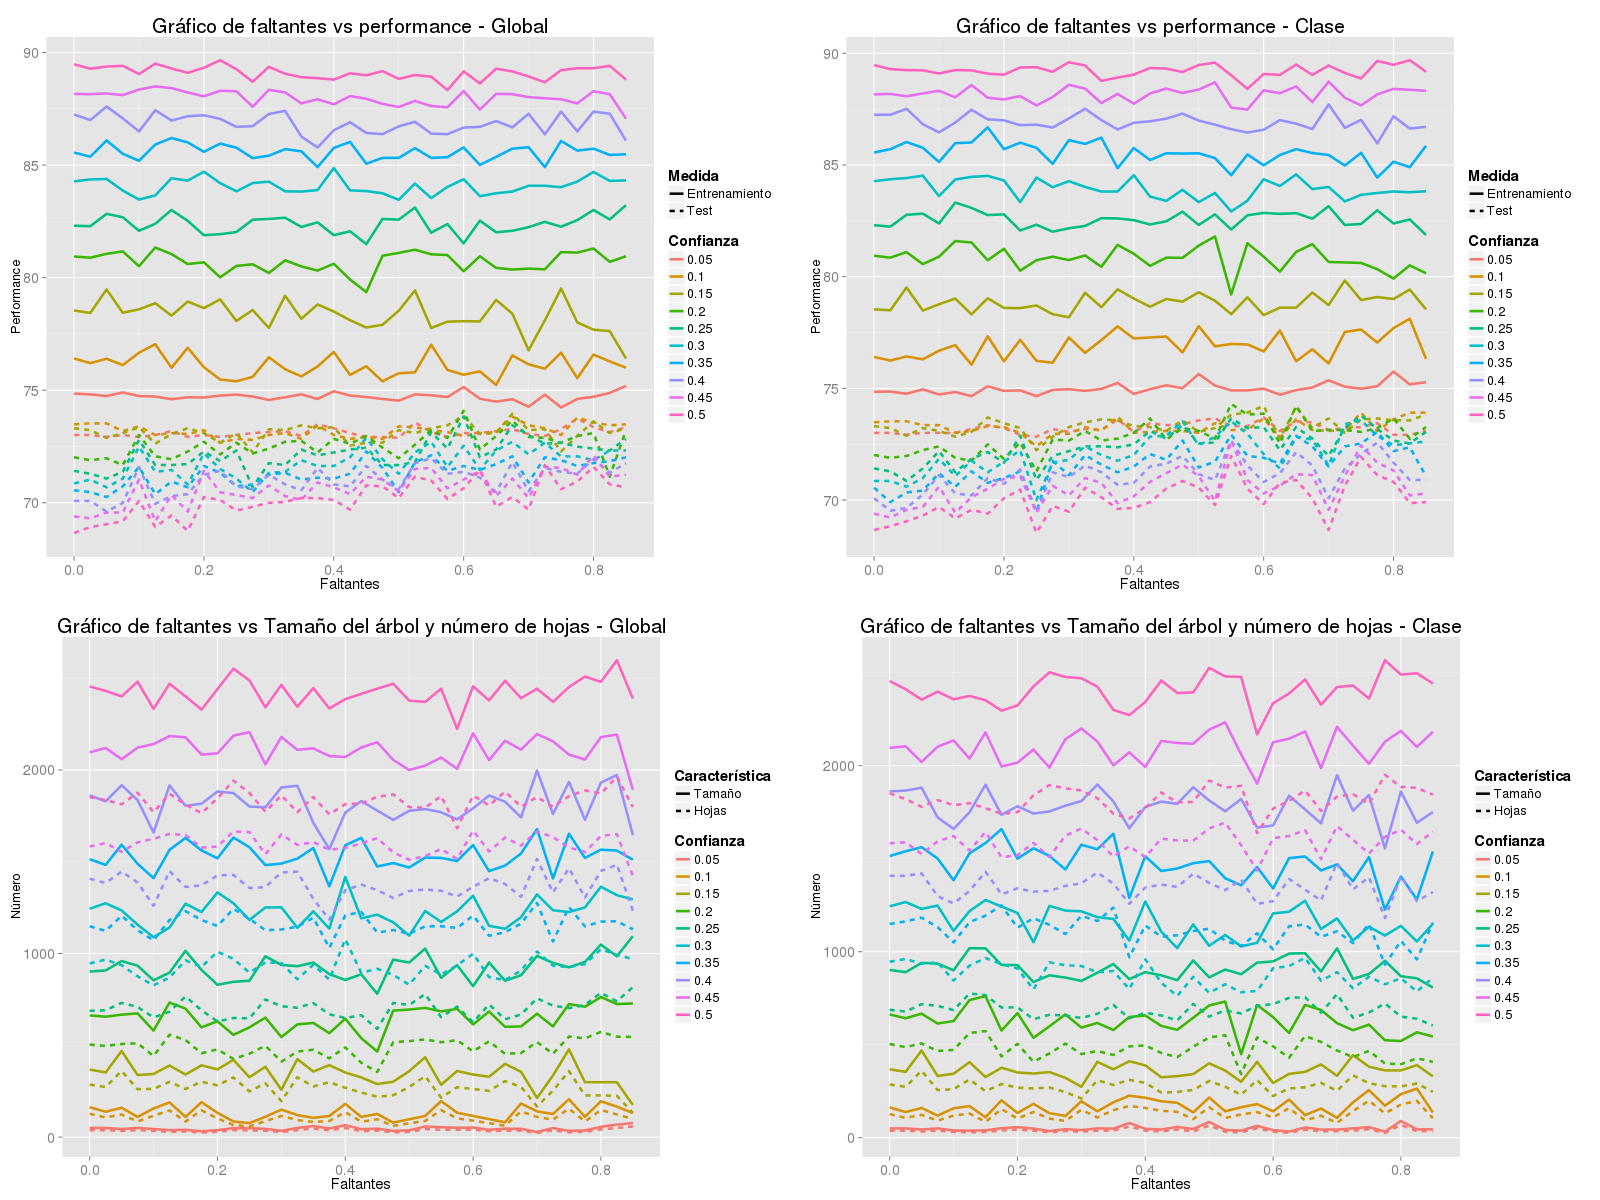
\includegraphics[scale = 0.27]{2_1_Mult_Col_Unic_Fil}
	\caption[Faltantes Múltiple variable]{Gráficos de Faltantes en Múltiples variables con un solo faltante por fila}
	\label{2.P2MultVarUnicFil}
\end{figure}

\subsubsection{Imputación sin tener en cuenta la clase}

\subsubsection{Imputación teniendo en cuenta la clase}

\subsection{Sobre varias variables con múltiples faltantes por fila}
Para el último análisis, se agregaron datos faltantes sobre el total de entradas de el conjunto de datos (total de filas por total de columnas). Figura \ref{1.P2MultVarMultFil}

\begin{figure}[H]
	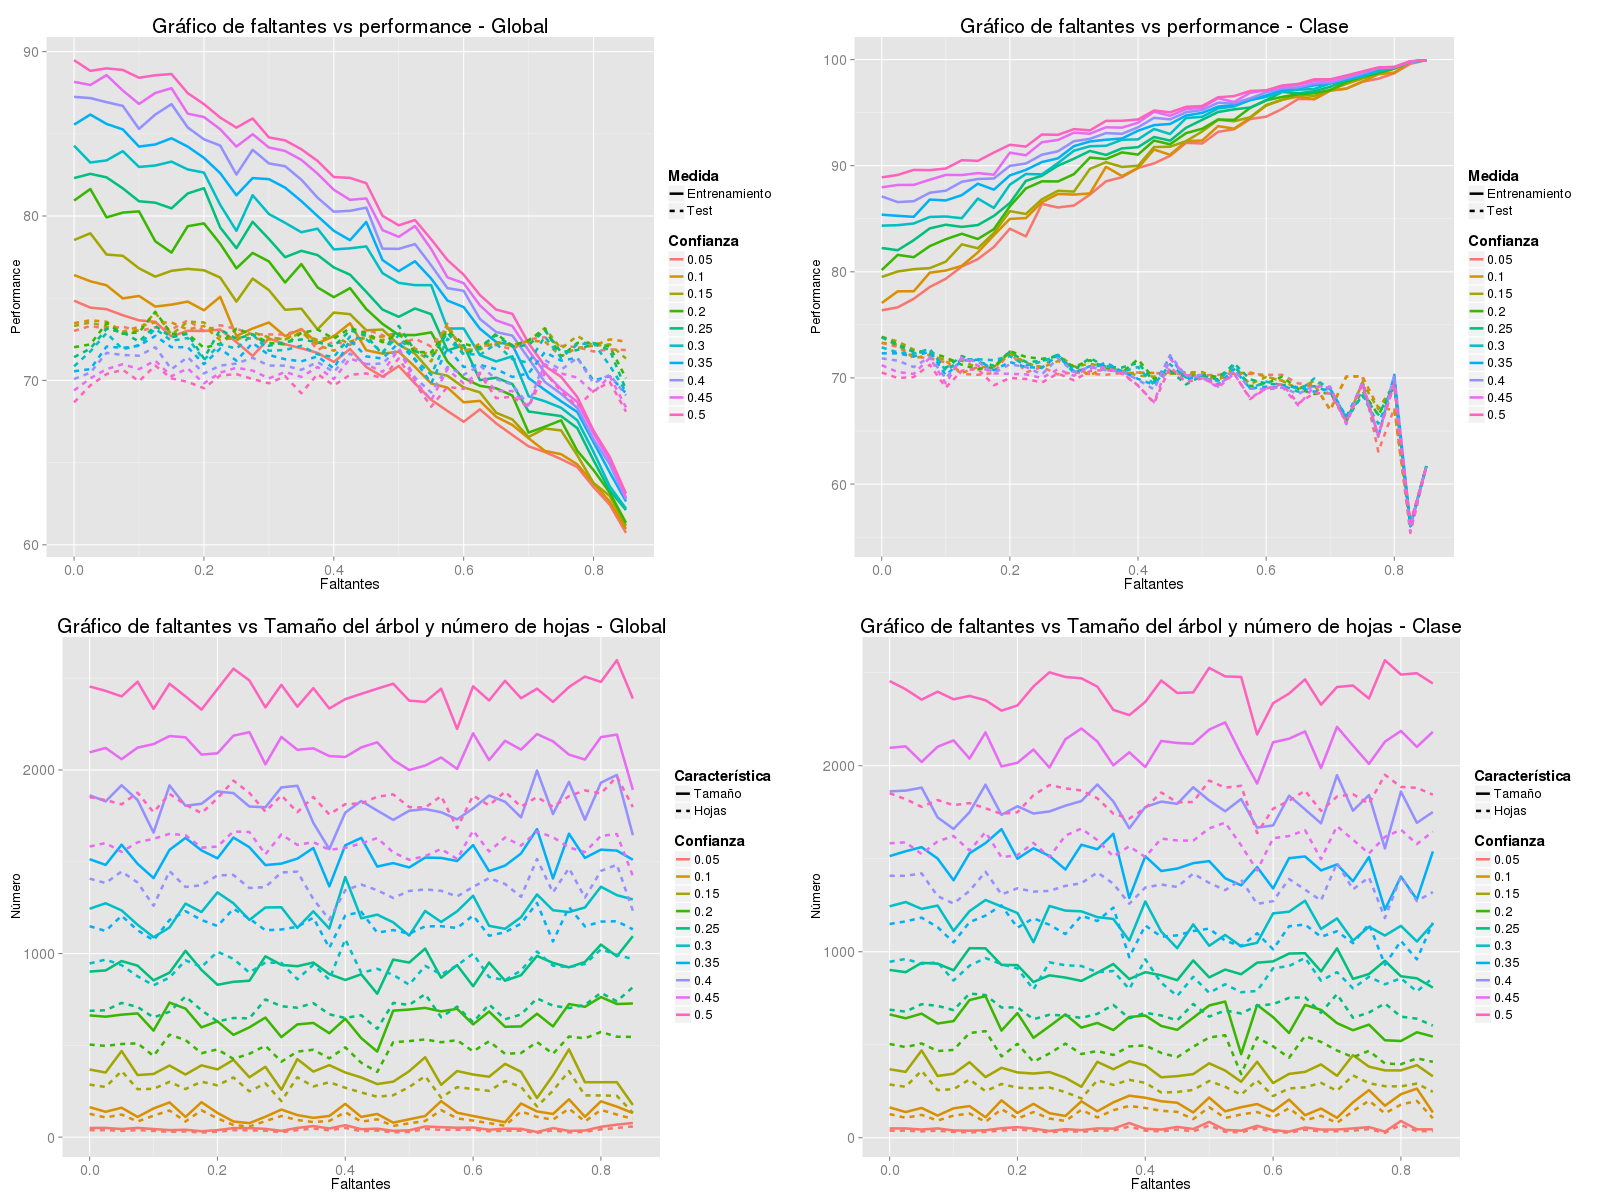
\includegraphics[scale = 0.27]{2_1_Mult_Col_Mult_Fil}
	\caption[[Faltantes Múltiples variables Múltiples Filas]{Gráficos de Faltantes en múltiples variables con múltiples faltantes por fila}
	\label{1.P2MultVarMultFil}
\end{figure}

\subsubsection{Imputación sin tener en cuenta la clase}

\subsubsection{Imputación teniendo en cuenta la clase}

\section{Tolerancia al ruido}
En esta parte, se genero entre 0 y 35\% de ruido sobre la clase. Figura \ref{3.P3Ruido}

\begin{figure}[H]
	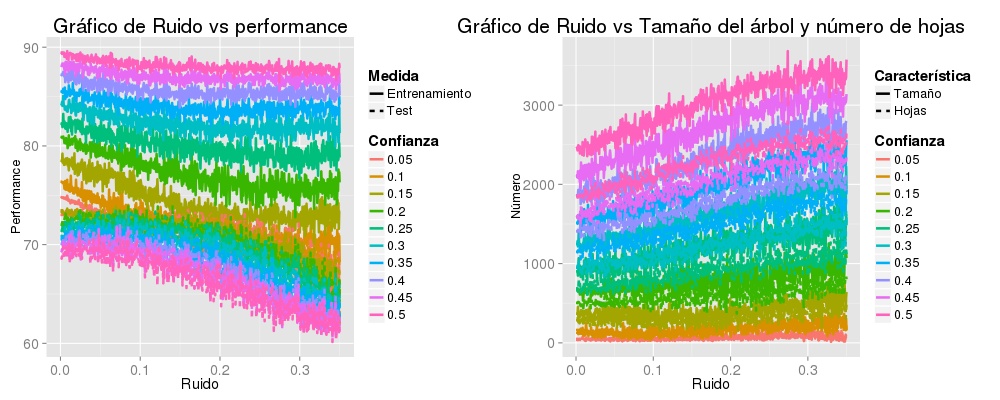
\includegraphics[scale = 0.4]{3_1_Ruido}
	\caption[Ruido]{Gráficos de Ruido}
	\label{3.P3Ruido}
\end{figure}

\section{Discretización de atributos numéricos}
La única variable numérica considerada es la EDAD ($S17$), que se procedió a discretizar según tres criterios para el diseño de las categorías: a) de igual densidad, b) de igual frecuencia, y c) supervisado, en base a la clase.

Si la variable a discretizar resultara relevante en términos de ganancia de información, se esperaría encontrar que a mayor cantidad de bins se incremente la performance del conjunto de entrenamiento. Para el caso, la variable EDAD evidencia poco aporte de información, independientemente del criterio de discretización utilizado. 

Para el ejercicio se programó una función que selecciona entre los distintos criterios y luego, para cada bin del intervalo $[1,20]$, se arma un dataset con la variable discretizada que se particiona en subconjuntos de entrenamiento ($80\%$) y test ($20\%$). Luego, para la familia de combinaciones de factor de confianza en el intervalo $[0.05,0.5]$ a pasos de $0.05$, se corre llama al J48 sobre el primer dataset para extraer el modelo a utilizar con el conjunto de test y de ambas corridas se extrae la información que se precisa: tamaño del árbol, cantidad de hojas y performance.

\subsection{Discretización por densidad}

En este caso, como se observa en la figura XX se encontró que la variable discretizada prácticamente no incide en la performance ni en en el tamaño del árbol, lo cual estaría indicando que es un atributo sin mayor poder de discriminación.

\subsection{Discretización por frecuencias}

En el caso de la discretización por frecuencias se observa una respuesta similar, con signos de independencia tanto del tamaño del árbol como de la performance respecto de la cantidad de bins de discretización. En comparación con el criterio anterior, aparentemente no introduce mejoras a la performance en el conjunto de entrenamiento. 

\subsection{Método supervisado}
Para este criterio, dado que no puede elegirse la cantidad de bines sino que es una salida de la corrida algoritmo, corresponde observar cuántos niveles utiliza el algoritmo en la discretización, que para el caso es uno solo. Con el dataset utilizado se observa que el J48 entrega una sola categoría (bin), que para la variable de clase no aporta nueva información.

\subsection{Sobre variables con poco poder discriminativo}

\begin{figure}[H]
	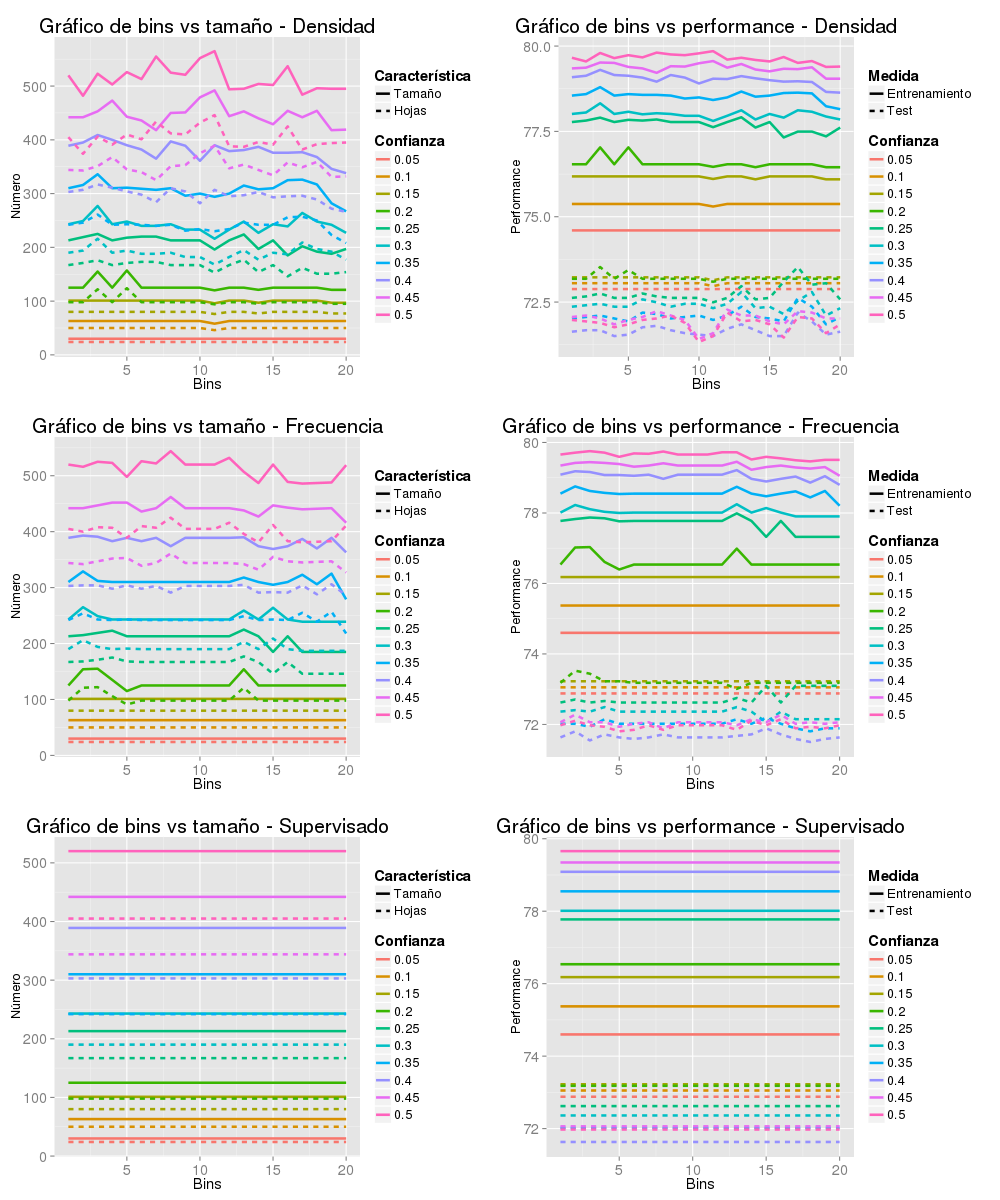
\includegraphics[scale = 0.4]{4_1_Bins_Todas_var}
	\caption[Ruido]{Gráficos de Ruido}
	\label{4.P4Todas}
\end{figure}


\subsection{Sobre variables con mucho poder discriminativo}

\begin{figure}[H]
	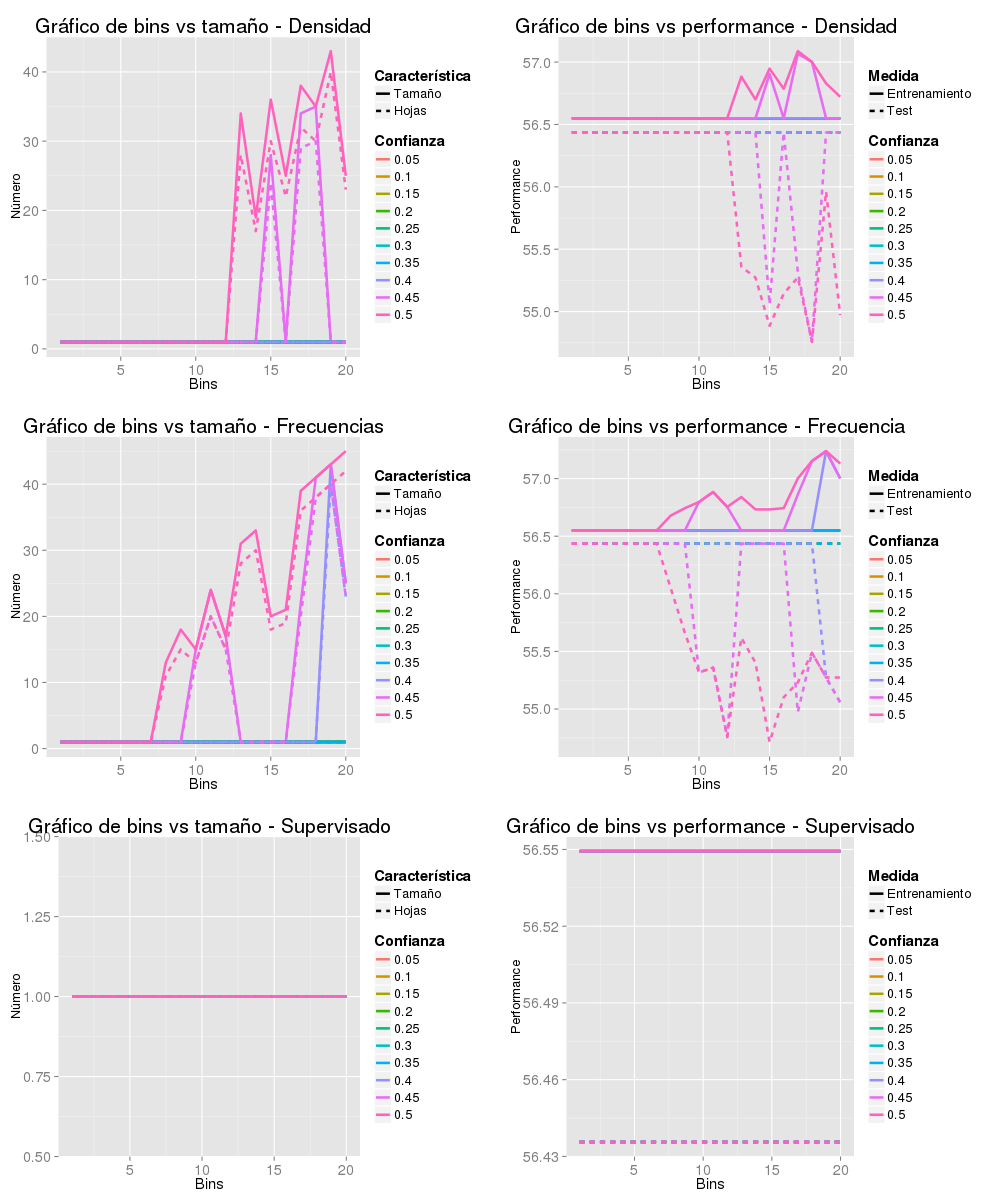
\includegraphics[scale = 0.4]{4_2_Bins_Selected_var}
	\caption[Ruido]{Categorización tenien}
	\label{4.P4Selected}
\end{figure}




\section*{Conclusiones}
Con respecto a los datos faltantes, el árbol tiene una tolerancia similar a la mayoría de métodos estadísticos, en donde se admite al rededor de un 20\% de datos faltantes. \\
En cuanto a la discretización de variables, en el ejercicio se observa claramente que la variable numérica seleccionada EDAD no aporta elementos determinantes en la predicción del valor de la clase. Al revisar su comportamiento discretizándola en un conjunto más reducido de variables con performance similar (con poca ganancia de información), en ningún momento forma parte del árbol, es decir que el algoritmo detecta el bajo poder de discriminación presente en la misma y la descarta lo cual resulta un comportamiento esperable.


\section*{Trabajo futuro}
Para poder verificar las propiedades del método para su aplicación en problemas de la vida real, sería conveniente mezclar las diferentes pruebas hechas sobre en este trabajo. ¿qué pasa cuando el árbol es sometido a ruido y a faltantes al mismo tiempo?. Además de esto, sería conveniente intentar otros métodos para imputación de datos categóricos que sesguen menos los datos, como por ejemplo el método de imputación Hot Deck, el cual, busca individuos similares al individuo con el dato faltante para "donarle" el dato que le hace falta. \cite{Rodgers1984}

\bibliographystyle{apalike}	
\bibliography{Bibliografia.bib}



%\section*{Referencias}

\end{document}
